
\begin{align}
y=\frac{x-1}{x-2}\label{eq:solutions/12/2.1}
\end{align}
Equation \eqref{eq:solutions/12/2.1} can be expressed as
\begin{align}
y(x-2)=x-1\\
yx-2y-x+1=0\label{eq:solutions/12/2.0.3}
\end{align}
From above we can say,
\begin{align}
\vec{V}=\frac{1}{2}\myvec{0 & 1\\ 1 & 0}\\
\vec{u}=\myvec{-\frac{1}{2}&-1}\\
f=1
\end{align}
Now,
\begin{align}
\because \abs{V} = \mydet{0& \frac{1}{2} \\ \frac{1}{2} & 0} < 0,
\end{align}
\eqref{eq:solutions/12/2.1} is the equation of a hyperbola. To verify that this we will find the the characteristic equation of $\vec{V}$.
\begin{align}
\mydet{\lambda \vec{I}-\vec{V}} = \mydet{\lambda  & \frac{1}{2}\\ \frac{1}{2} & \lambda } &= 0
\\
\implies \lambda^2 - 2\lambda + \frac{3}{4} &= 0
\label{eq:solutions/12/2.0.13}
\end{align}
The eigenvalues are the roots of \eqref{eq:solutions/12/2.0.13} given by
\begin{align}
\lambda_1 = \frac{1}{2}, \lambda_2 = -\frac{1}{2}
\label{eq:solutions/12/2.0.14}
\end{align}
The eigenvector $\vec{p}$ is defined as
\begin{align}
\vec{V} \vec{p}&= \lambda \vec{p}
\\
\implies \brak{\lambda\vec{I}-\vec{V}}\vec{p} &=0
\end{align}
where $\lambda$ is the eigenvalue.  For $\lambda_1 = \frac{1}{2}$,
\begin{align}
\brak{\lambda_1\vec{I}-\vec{V}}
= \myvec{\frac{1}{2} & \frac{1}{2}
\\ \frac{1}{2} & \frac{1}{2}} 
\xleftrightarrow[R_1 \leftarrow 2R_1] {R_2\leftarrow R_2-R_1}\myvec{1 & 1 \\0 & 0 }  
\\
\implies \vec{p}_1 = \frac{1}{\sqrt{2}}\myvec{1 \\- 1}
\end{align}
Now,$\lambda$ is the eigenvalue.  For $\lambda_2 = -\frac{1}{2}$,
\begin{align}
\brak{\lambda_2\vec{I}-\vec{V}}
= \myvec{-\frac{1}{2} & \frac{1}{2}
\\ \frac{1}{2} & -\frac{1}{2}} 
\xleftrightarrow[R_1 \leftarrow 2R_1] {R_2\leftarrow R_2+R_1}\myvec{-1 & 1 \\0 & 0 }  
\\
\implies \vec{p}_2 = \frac{1}{\sqrt{2}}\myvec{1 \\ 1}
\end{align}
From Equations,
\begin{align}
\vec{V} &= \vec{P}\vec{D}\vec{P}^{-1}=\vec{P}\vec{D}\vec{P}^T \quad \because \vec{P}^{-1} = \vec{P}^{T}
\\
\text{or, } \vec{D} &= \vec{P}^T\vec{V}\vec{P}
\end{align}
We can say that
\begin{align}
\vec{P} & =\myvec{\vec{p}_1 & \vec{p}_2} = \frac{1}{\sqrt{2}}\myvec{1 & -1\\ 1 & 1}\\
 \vec{D} &= \myvec{\lambda_1 & 0 \\ 0 & \lambda_2} =\myvec{\frac{1}{2} & 0\\ 0 & -\frac{1}{2}}
\end{align}
$\because \vec{u}^T\vec{V}^{-1}\vec{u}-f > 0 ,$there isn't a need to swap axes.
In hyperbola,
\begin{align}
\vec{c}=-\vec{V}^-1\vec{u}\\
axes=
\begin{cases}
\sqrt{\frac{\vec{u}^T\vec{V}^{-1}\vec{u}-f}{\lambda_1}}\\ \sqrt{\frac{f-\vec{u}^T\vec{V}^{-1}\vec{u}}{\lambda_2}}
\end{cases}
\end{align}
From above equations we can say that,
\begin{align}
\vec{c}=\myvec{-2\\-1}\\
\sqrt{\frac{\vec{u}^T\vec{V}^{-1}\vec{u}-f}{\lambda_1}}=\sqrt{2}\\
\sqrt{\frac{f-\vec{u}^T\vec{V}^{-1}\vec{u}}{\lambda_2}}=\sqrt{2}
\end{align}
with the standard hyperbola equation becoming
\begin{align}
\frac{x^2}{2}-\frac{y^2}{2} = 1,
\label{eq:solutions/12/2.0.30}
\end{align}
Let us assume slope to be l,now finding the direction vector and normal vector of the tangent with slope l.
\begin{align}
\vec{m}=\myvec{1\\l}\label{eq:solutions/12/2.0.27}\\
\vec{n}=\myvec{l\\-1}\label{eq:solutions/12/2.0.28}
\end{align}
Now considering the equations to find point of contact
\begin{align} \vec{q} = \vec{V}^{-1}\brak{\kappa \vec{n}-\vec{u}}\label{eq:solutions/12/2.0.33}
\\
\kappa = \pm \sqrt{\frac{\vec{u}^T\vec{V}^{-1}\vec{u}-f}{\vec{n}^T\vec{V}^{-1}\vec{n}}} \label{eq:solutions/12/2.0.34}
\end{align}
By using \eqref{eq:solutions/12/2.0.34}
\begin{align}
\kappa=\sqrt{-\frac{1}{4l}}
\end{align}
Now substituting this $\kappa$ in \eqref{eq:solutions/12/2.0.33}
\begin{align}
\vec{q}=\myvec{-2\sqrt{-\frac{1}{4l}}+2\\2\sqrt{\frac{-l}{4}}+1}
\end{align}
We know that x=10.
\begin{align}
-2\sqrt{-\frac{1}{4l}}+2=10\\
-2\sqrt{-\frac{1}{4l}}=8\\
\sqrt{-\frac{1}{4l}}=4\\
-\frac{1}{4l}=16\\
l=-\frac{1}{64}
\end{align}
The slope of the tangent to the curve y=$\frac{x-1}{x-2}$, x$\not=$2 at x=10 is $\frac{1}{64}$.
So,from the above we can say that $\kappa$=4,-4 and from equation \eqref{eq:solutions/12/2.0.27} and \eqref{eq:solutions/12/2.0.28} direction and normal vectors will come out to be
\begin{align}
\vec{m}=\myvec{1\\-\frac{1}{64}}\\
\vec{n}=\myvec{-\frac{1}{64}\\-1}
\end{align}
Now using equation \eqref{eq:solutions/12/2.0.33}
\begin{align}
\vec{q}_1 = \vec{V}^{-1}\brak{\kappa_1 \vec{n}-\vec{u}}\\
\vec{q}_1 = \myvec{0&2\\2&0}\brak{-4 \myvec{-\frac{1}{64}\\-1}-\myvec{-\frac{1}{2}\\-1}}\\
\vec{q}_1=\myvec{10\\ \frac{9}{8}}\\
\vec{q}_2 = \vec{V}^{-1}\brak{\kappa_2 \vec{n}-\vec{u}}\\
\vec{q}_2 = \myvec{0&2\\2&0}\brak{4 \myvec{-\frac{1}{64}\\-1}-\myvec{-\frac{1}{2}\\-1}}\\
\vec{q}_2=\myvec{-6\\ \frac{7}{8}}
\end{align}
  \begin{figure}[h!]
	\centering
	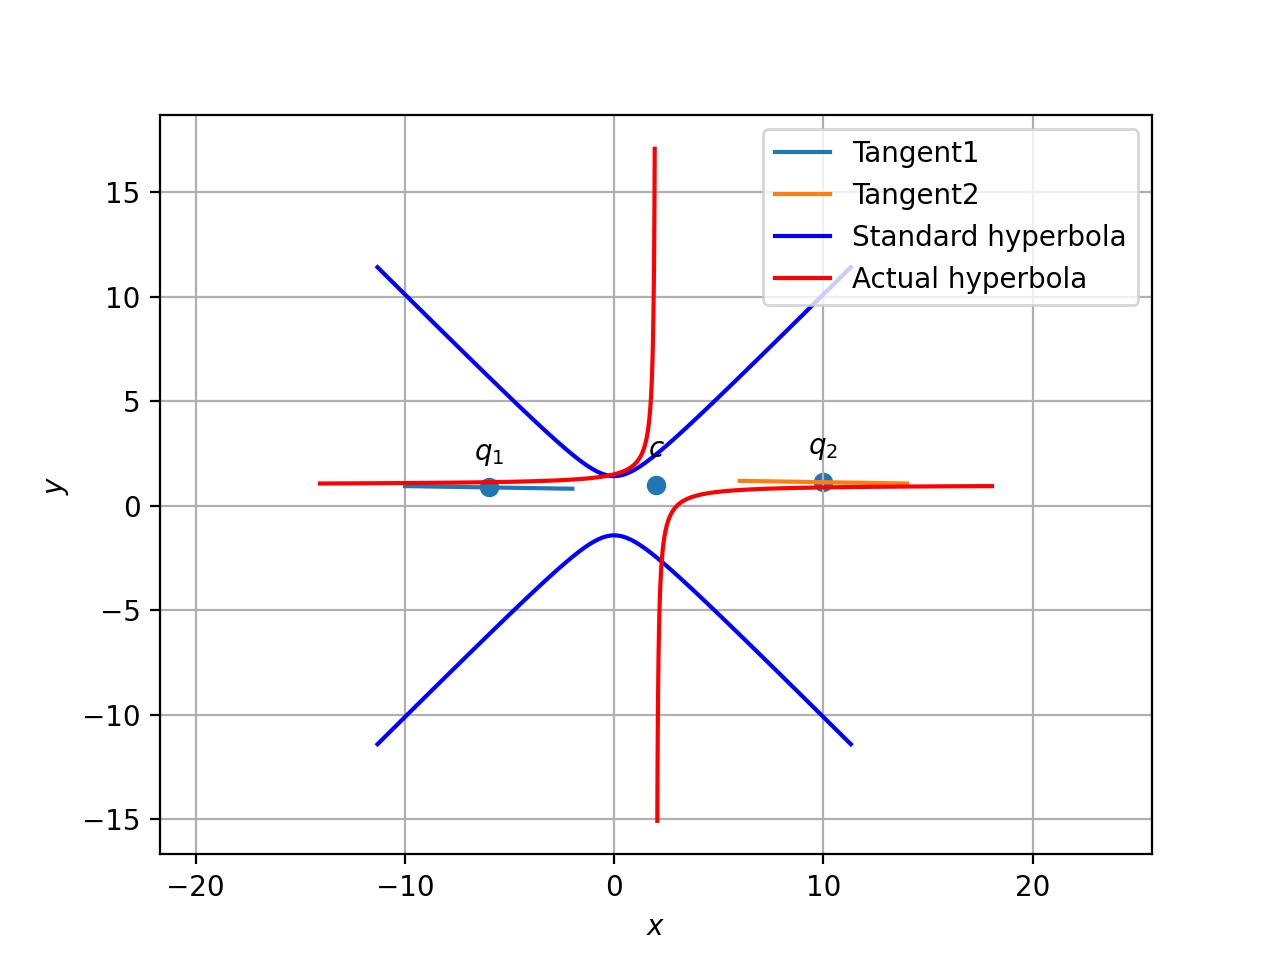
\includegraphics[width=\columnwidth]{./solutions/1/12/Assignment_7.png}
	\caption{Tangent 2 shows the tangent}
	\label{eq:solutions/12/myfig}
\end{figure}
